\documentclass{article}
\title{Discussions about the project during ``UCA School on Complex systems 2021''}
\usepackage{amsmath,amssymb,amsfonts}
\usepackage{graphicx,tikz}
\usetikzlibrary{patterns}
\usepackage{url}
\usepackage{algorithm,algorithmic}
\usepackage{fullpage}
\author{L. Berti, Z. El Kiyati, S. Reidel; L. Giraldi, C. Prud'homme}

\newcommand{\qhat}{\hat{Q}}
\begin{document}
	\maketitle
	\section{19 October}
	\subsection{Three sphere swimmer far from walls}
	Possible actions
	\begin{itemize}
		\item Shrink 1 arm
		\item Elongate 1 arm
	\end{itemize}
	Possible States
	\begin{itemize}
		\item $(L_1,L_2) \in \{A,B\}^2$ with $A, B$ fixed values
	\end{itemize}
	Reward
	\begin{itemize}
		\item $\delta_t = X^{CM}_{t+1}-X_t^{CM}$ every step
		\item $R = \sum_t \gamma^t\delta_t$ cumulative reward
	\end{itemize}
	Procedure for reinforcement learning that was followed:
	\begin{itemize}
		\item Start with state $s_t$ and action $a_t$ (chosen via Q-learning)
		\item Simulate passing between $s_t$ and $s_{t+1}$ as specified by $a_t$ in unit time
		\item Update the Q-function with the rule $Q^\pi(s_t,a_t) \leftarrow Q^\pi(s_t,a_t) + \alpha(r_t + \gamma \max_a Q^\pi(s_{t+1},a)-Q^\pi(s_{t},a_{t})).$
	\end{itemize}
	Precise values we looked at (during M2 project): 
	\begin{itemize}
		\item R=1 radius of the spheres
		\item B=10 maximal length of the arms
		\item A=6 minimal length of the arms
		\item $\Delta=0.16R$ Displacement after one swimming period (L=Long Arm, S=Short Arm; Sequence during swimming period: LL, SL, SS, LS, LL)
	\end{itemize}
\begin{figure}
	\centering
	\resizebox{0.45\linewidth}{!}{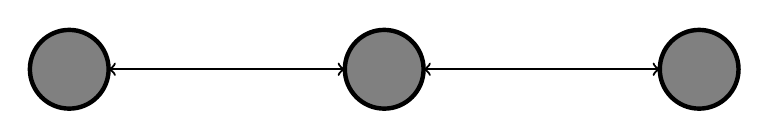
\begin{tikzpicture}
			\draw[ultra thick,, fill=gray]  (-4,0) ellipse (0.5cm and 0.5cm);
			\draw[ultra thick,, fill=gray]  (0,0) ellipse (0.5cm and 0.5cm);
			\draw[ultra thick,, fill=gray]  (4,0) ellipse (0.5cm and 0.5cm);
			\draw[thick,<->] (-3.5,0) -- (-0.5,0);
			\draw[thick,<->] (3.5,0) -- (0.5,0);
%			\draw[ ultra thick,-] (-4.5,-2) -- (4.5,-2);
%			\draw[pattern=north east lines, pattern color=black] (-4.5,-2) rectangle (4.5,-4);
	\end{tikzpicture}}
\caption{Three sphere swimmer, far from walls.}
\end{figure}
\subsection{Three sphere swimmer next to a wall}
Experimentally, swimmers have high affinity to the walls, they stick to it. Then, depending on the angle, they can be deflected.

We discussed about different aspects to describe our problem:

\paragraph{Reward:} Swim in the $x$ direction and, at the same time, try to maintain the distance $H$ from the wall
\[
r_t=\frac{(\vec{X}_{CM}^{t+1}-\vec{X}_{CM}^t)\cdot \hat{e}_x}{|y_{CM}-H|}
\]
\paragraph{Actions:} Discrete action space, where you can choose how much you can shrink your arm
\[
A = \{2,4,6,8\} \quad\text{Supposing that the initial length is 10}
\]
The way to deal with continuous actions spaces is to put a probability distribution over the space, learn it and use it to choose the future states. A possible algorithm is Normalised Advantage Function (NAF). However, it is sensibly more difficult than ``just'' continuous state spaces.
\begin{figure}
	\centering
	\resizebox{0.45\linewidth}{!}{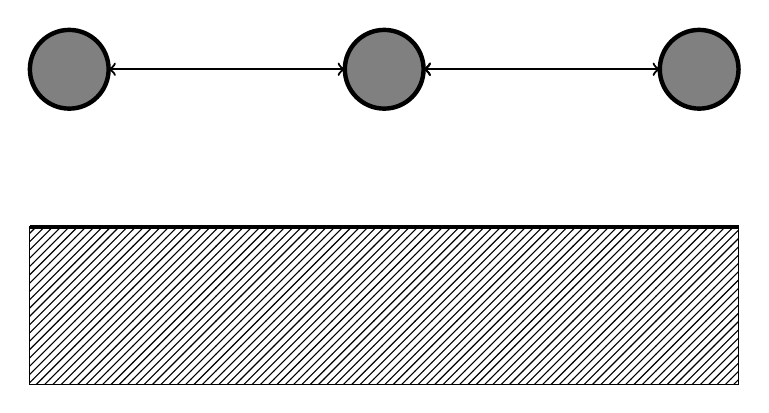
\begin{tikzpicture}
			\draw[ultra thick,, fill=gray]  (-4,0) ellipse (0.5cm and 0.5cm);
			\draw[ultra thick,, fill=gray]  (0,0) ellipse (0.5cm and 0.5cm);
			\draw[ultra thick,, fill=gray]  (4,0) ellipse (0.5cm and 0.5cm);
			\draw[thick,<->] (-3.5,0) -- (-0.5,0);
			\draw[thick,<->] (3.5,0) -- (0.5,0);
			\draw[ ultra thick,-] (-4.5,-2) -- (4.5,-2);
			\draw[pattern=north east lines, pattern color=black] (-4.5,-2) rectangle (4.5,-4);
			\draw[thick,->] (3.5,0) -- (0.5,0);
			\draw[thick,->] (3.5,0) -- (0.5,0);
	\end{tikzpicture}}
	\caption{Three sphere swimmer, close to a wall.}
\end{figure}
\paragraph{States:} (in other words, the states describing the swimmer)
\begin{itemize}
	\item Mass centres of the spheres $(X_{CM}^1,X_{CM}^2,X_{CM}^3)$
\end{itemize}
NB: the orientation of the swimmer can be computed using the centres of mass, as well as the distance from the wall (and in principle also the lengths of the arms). However, when looking at function approximation, inputting also these other variables might help learning.
\\

\emph{\textbf{Question:} Does the problem have the Markov property (i.e. $\mathbb{P}[s_{t+1}|s_0,a_0,s_1,a_1,\dots,s_t,a_t,]= \mathbb{P}[s_{t+1}|s_t,a_t]$)? Depending on the state that describes the problem, it might or might not have it.
A way to check this is to test the independence of the future with respect to the past via a test of independence. The test is the following: 
\begin{itemize}
	\item Take a collection of samples of your state $s_t =(X_{CM}^1,X_{CM}^2,X_{CM}^3)$ in a discrete  set $\{a,b,c,\dots\}$
	\item Compute the evolution of your collection of samples
	\item Realise a test of independence via a $\chi^2$ test $\forall x \in \{a,b,c,\dots\}$ of the past and future, i.e. $(s_{i-1},s_{i+1})$ and verify you always have a positive result. If not, the process does not have the Markov property as the future is not independent from the past.
\end{itemize}}
\paragraph{Discretization of the problem?}If we suppose the Markov property, we could think in a first approximation to discretise the state space and attempt a Q-learning algorithm (i.e. matrix representation of the $Q$-value function). The idea is to build a grid over the $xy$ plane and use the midpoint of each square as the approximation every time the continuous state variable happens to fall in the square.

However, since the state corresponds to the three centres of mass of the sphere, each in $\mathbb{R}^2$, the size of the discretized state space rapidly explodes if we want to make a good discretization of the 2d region in which the swimmer evolves.
\paragraph{Continuous state problem.} In this case, we allow the state variables (centres of mass of the three spheres) to vary continuously in spaces of the form $[A_i,B_i]\times[C_i,D_i]$, for $i=1,2,3$.
\begin{enumerate}
\item The first approach we will look at is  a \emph{\textbf{linear function approximation of $Q$}} of the form $Q(s,a)\approx\hat{Q}(s,a;w) = <x(s,a),w>$ where $\hat{Q}$ is the approximation of $Q$, $w$ are the weights of the linear estimator, $x(s,a)$ are feature vectors (i.e. combinations of state and action that best describe our problem).

In this first approach, we will look at an episodic treatment of our problem: we fix a ``finish line'' at $X=0.5$, for example, and we reward the swimmer based on the velocity with which this finishing line is attained. The best policy we will look for will be the one allowing to get there faster. We ask
\begin{itemize}
	\item $|X_{t_F}-x_{CM,t_0}|>0.5$  
	\item a the same time, fix a maximal time for which one episode is allowed to run, for example $t \le 10 T$ where $T$ is the cycle period of the swimming stroke. 
\end{itemize}
The communication with the fluid solver is always performed by reading the result file (to get the centres of mass) and by modifying the input files (to prescribe the new action) until the final total time is reached, and this for each episode.
\item The second approach we will look at is the \emph{\textbf{non-linear function approximation}} of $Q$ using neural networks. During our investigation, we will try with Deep Q-Network (inspired by paper \cite{novati_synchronisation_2017}) and with Deep Q-network with Long-Short Term Memory layers (inspired by paper \cite{verma_efficient_2018}).
\end{enumerate}
\section{20 October}
\subsection{Linear continuous model}
The first step now is to construct the \textit{feature vector} $x(s,a)$, function fo the state and actions that should encode some sort of interaction informations at the input of the model. In order to do so, we chose a tiling code approach (see \cite[Section 9.5]{sutton_reinforcement_2018}) that uses a finite collection of tiling square patterns to locate regions in the continuous space where the update of the $Q$ function should be ``extended''. 

A tiling code algorithm is proposed in Python by R. Sutton in its website\footnote{\url{http://incompleteideas.net/tiles/tiles3.html}}. It outputs a vector $v$ of $N_{tilings}$ components, whose value $v_i$ is the global index of the tile among the whole collection of tiles, and at the same tile belongs to tiling $i$. 

Once the feature vector has been constructed via tiling code, we apply an episodic semi-gradient\footnote{``Semi-gradient'' because there is not a gradient term with respect to weights of $\qhat(S',A';w)$, and a not a complete gradient of the $(R+\qhat(S',A';w)-\qhat(S,A;w))^2$ loss function is computed.} SARSA method to approximate the $Q$ function with a linear model $\qhat$ \cite[Sec 10.1]{sutton_reinforcement_2018} as reported in \ref{Algo:semi-gradientSARSA}. In the algorithm, $\qhat(s,a;w) = <x(s,a),w>$ is the linear approximation of the $Q$ function, hence $\nabla_w \qhat = x(s,a)$.
\begin{algorithm}
	\begin{algorithmic}
		\REQUIRE $\alpha>0,\epsilon>0, w\in \mathbb{R}^d$, $\qhat$ parametrization (linear for us)\\		
		\FOR{$i$ in $N_{episodes}$}
		\STATE{Choose $S,A$ initial state and action of the episode (use $\epsilon$-greedy)\\
		\FOR{$j$ in $N_{step}$}
		\STATE{Take action $A$ and observe $S',R$\\
		\IF{$S'$ is terminal}
		\STATE{$w \leftarrow  w + \alpha[R-\qhat(S,A;w)]\nabla_w \qhat(S,A;w)$\\
		Go to next episode}
		\ENDIF\\
		Choose $A'$ as a function of $\qhat(S',\cdot;w)$ via $\epsilon$-greedy scheme\\
		$w \leftarrow  w + \alpha[R+\gamma \qhat(S',A';w)-\qhat(S,A;w)]\nabla_w \qhat(S,A;w)$\\
		$S \leftarrow S'$\\
		$A\leftarrow A'$
		}
		\ENDFOR
		}
		\ENDFOR
		\ENSURE $w$
	\end{algorithmic}
\caption{Episodic semi-gradient SARSA approximation of $\qhat$}
\label{Algo:semi-gradientSARSA}
\end{algorithm}
\bibliography{bib_UCA_school_project}
\bibliographystyle{siam}
\end{document}